\documentclass[11pt,twoside,a4paper]{book}
\usepackage[utf8]{inputenc}
\usepackage[english]{babel}
\usepackage{caption}
\usepackage{subcaption}
\usepackage{minted}
\usepackage{amssymb}
\usepackage{mathtools}
\usepackage{listings}
\usepackage{graphicx}
\usepackage{hyperref}
\usepackage[dvipsnames,hyperref]{xcolor}
\usepackage{pdfpages}
\usepackage{caption}
\usepackage{csquotes}
\usepackage[style=numeric,citestyle=ieee,hyperref,natbib,backend=biber]{biblatex}
\addbibresource{reference.bib}

\definecolor{aliceblue}{RGB}{240,248,255}
\definecolor{wonderland}{RGB}{15,123,196}
\hypersetup{%
    colorlinks=true, linktocpage=true, pdfstartpage=1, 
    pdfstartview=FitV, breaklinks=true, pdfpagemode=UseNone, 
    pageanchor=true, pdfpagemode=UseOutlines,%
    plainpages=false, bookmarksnumbered,
    bookmarksopen=true,%
    bookmarksopenlevel=1,%
    hypertexnames=true, pdfhighlight=/O,%
    urlcolor=wonderland,
    linkcolor=RoyalBlue, 
    citecolor=wonderland,%
    hyperfootnotes=false,
    pdfpagelabels,
    pdfsubject={},%
    pdfkeywords={},%
    pdfcreator={pdfLaTeX},%
    pdfproducer={LaTeX}%
}

\let\tmp\oddsidemargin
\let\oddsidemargin\evensidemargin
\let\evensidemargin\tmp
\reversemarginpar

\usepackage{titlesec}
\usepackage{xcolor}
\usepackage{fancyhdr}
\usepackage{graphicx}
\usepackage{titling}

\definecolor{darkaccent}{HTML}{007AC2}
\definecolor{lightaccent}{HTML}{107AC2}

%page style
\pagestyle{fancy}
\renewcommand{\headrulewidth}{0pt}
\renewcommand{\footrulewidth}{0pt}

%section
\titleformat{\section}
[hang]
{\Large\bfseries}
{
\color{darkaccent}
\raisebox{-2pt}{
    \rule{0.35cm}{1em}
}
\color{black}
\sffamily
\thesection
}
{10pt}
{
\color{lightaccent}
\sffamily
\Large\bfseries
}
 
%subsection
\titleformat{\subsection}
[hang]
{\large\bfseries}
{
\color{darkaccent}
\raisebox{-2pt}{
    \rule{0.35cm}{1em}
}
\color{black}
\sffamily
\thesubsection
}
{10pt}
{
\color{lightaccent}
\sffamily
\large\bfseries
}

%subsubsection
\titleformat{\subsubsection}
[hang]
{\normalsize\bfseries}
{
    \empty
}
{10pt}
{
\color{darkaccent}
\raisebox{-2pt}{
    \rule{0.35cm}{1em}
}
\color{black}
\sffamily
\thesubsubsection
\color{lightaccent}
\hspace{1em}
\normalsize\bfseries
}
 
%chapter
\titleformat
{\chapter} 
[display] 
{\bfseries\huge} 
{
    \color{darkaccent}
    \raisebox{0em}{
        \rule{0.35cm}{1em}
    }
    \color{black}
    \sffamily
    \chaptertitlename \ \Huge\thechapter
} 
{-0.75em}
{
    \color{darkaccent}
    \raisebox{-2pt}{
        \rule{0.35cm}{1.5em}
    }
    \sffamily
    \color{lightaccent}
}

\renewcommand{\maketitle}
{
    \begingroup % Create the command for including the title page in the document
    \hbox
    { % Horizontal box
        \color{darkaccent}
        \rule{0.35cm}{\textheight} % Vertical line
        \color{black}
        \hspace*{0.05\textwidth} % Whitespace between the vertical line and title page text
        \parbox[b]{0.9\textwidth}
        { % Paragraph box which restricts text to less than the width of the page
            
            \noindent\sffamily\large\textbf{\TypeOfWork}\vspace{\baselineskip}\\
            
            \begin{tabular}{lc}
                
\includegraphics[width=3cm]{ctulogo} & 
                
                \color{lightaccent}\sffamily\Large\textbf{
                    \parbox[b]{5cm}{
                        České \\
                        vysoké\\
                        učení technické\\
                        v Praze
                    }
                    \vspace{1em}
                } \\
                \Huge\color{lightaccent}\sffamily\textbf{F3} & 
                \parbox[b]{5cm}{
                    \textbf{\Faculty} \\
                    \textbf{\Department}
                }
            \end{tabular}
            \vspace{3cm}
            
            \color{lightaccent}\sffamily\huge\textbf{\WorkTitle}\\
            
            \Large\color{black}\textbf{\FirstandFamilyName} \\
            \normalsize\textbf{\StudProgram} \\

            \vspace{6.5cm}
            
            \normalsize
            \textbf{\Date}\\
            \labelSupervisor: \Supervisor
        }
    }
    \endgroup
}

\newcommand{\splitpage}[3]{
    \begingroup
    \begin{center}
    \color{lightaccent}\huge\sffamily\centering\textbf{#1}
    \end{center}
    \raisebox{0.83\textheight}{\parbox[t]{0.45\textwidth}{
        #2
    }}
    \color{darkaccent}
    \hspace{1mm}
    \rule{0.35cm}{0.85\textheight} % Vertical line
    \hspace{1mm}
    \color{black}
    \raisebox{0.83\textheight}{\parbox[t]{0.45\textwidth}{
        #3
    }}
    \endgroup
} %Template

\author{Jan Dryk}

\newcommand\Date{\today}
\newcommand\Department{Department of Computer Science}
\newcommand\Faculty{Faculty of Electrical Engineering}
\newcommand\University{Czech Technical University in Prague}
\newcommand\SupervisorLabel{Supervisor}
\newcommand\StudyProgramLabel{Program}
\newcommand\StudyBranchLabel{Branch}
\newcommand\TypeOfWork{Diploma Thesis}
\newcommand\StudyProgram{Open Informatics}
\newcommand\StudyBranch{Software Engineering}
\newcommand\WorkTitle{An extension of  Process Simulate for optimization of robotic cells}
\newcommand\Author{Jan Dryk}
\newcommand\Supervisor{Ph.D. Přemysl Šůcha}


\begin{document}
\pagenumbering{gobble}
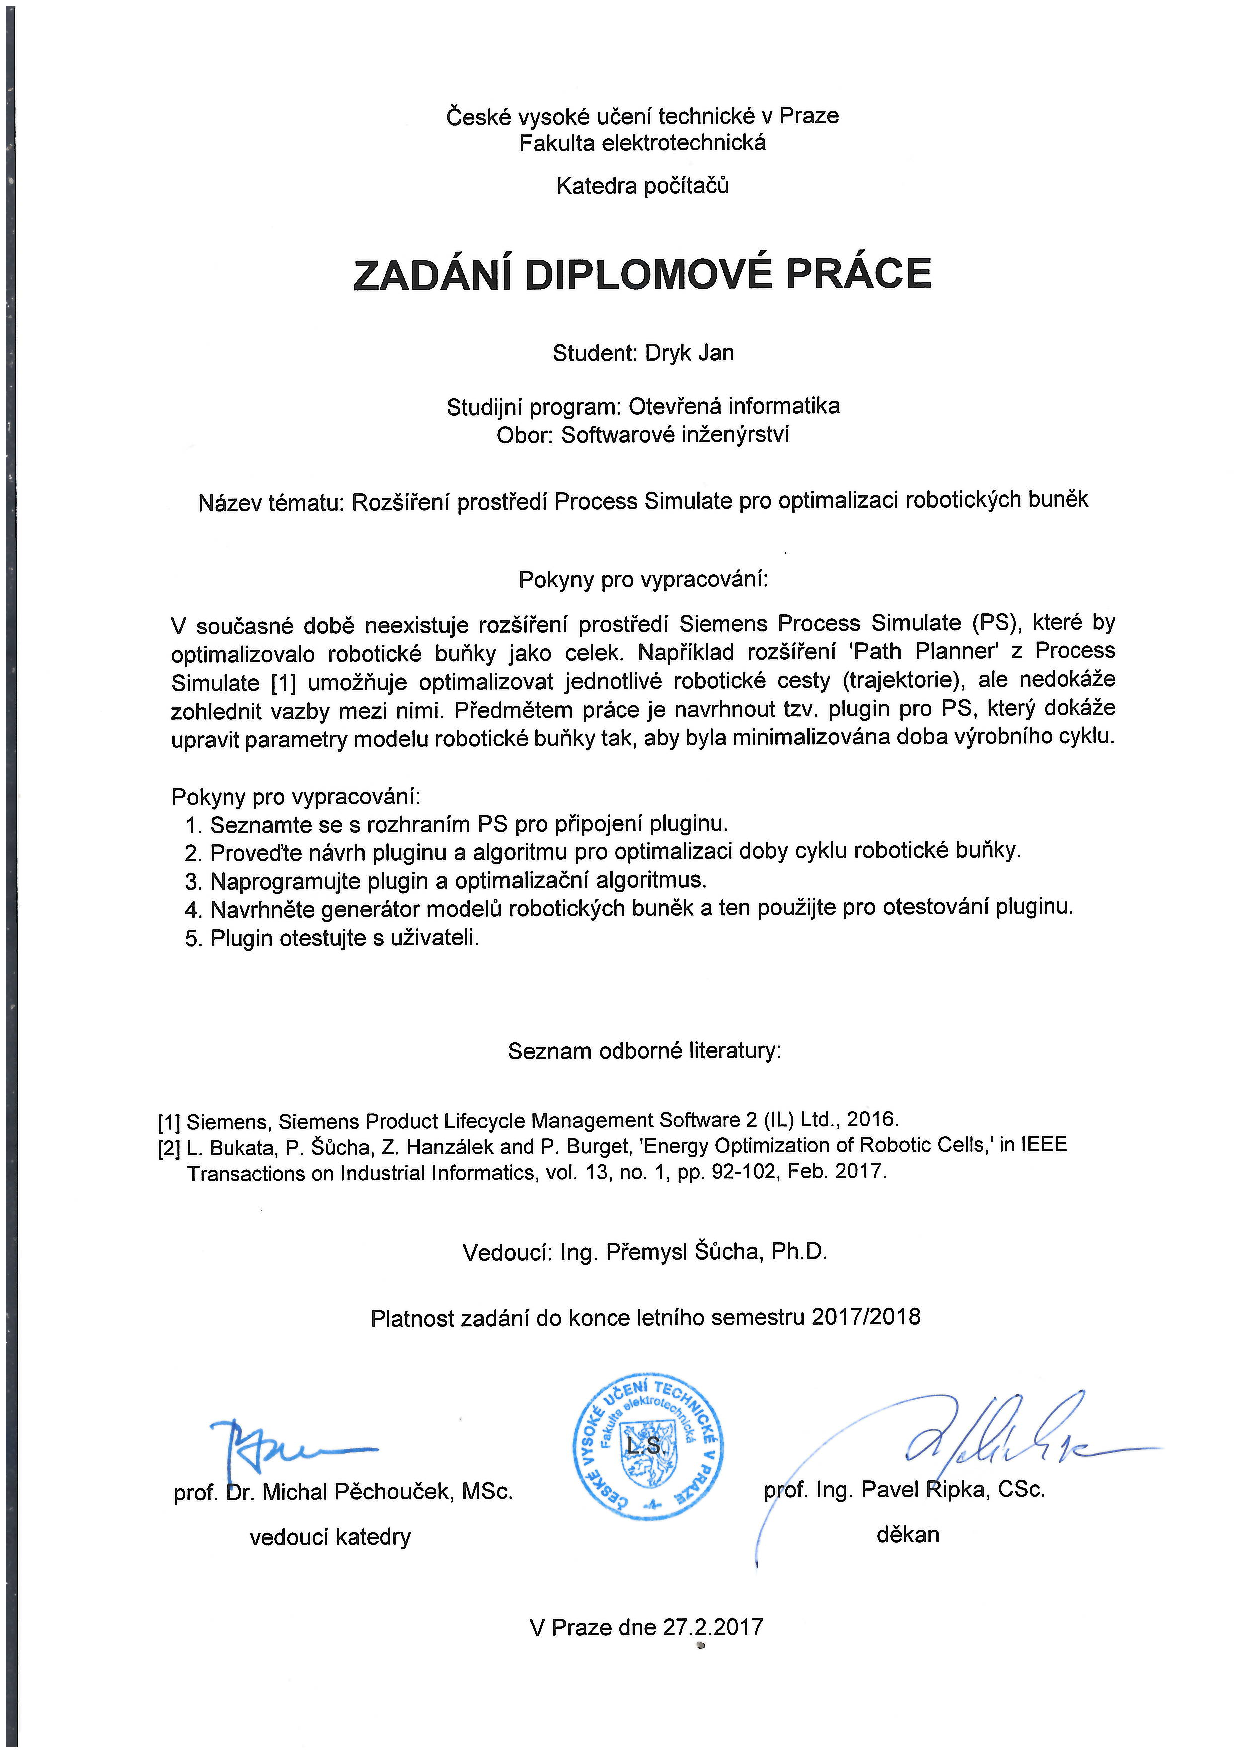
\includepdf{zadani.pdf}
\cleardoublepage

\pagenumbering{roman}
%Title page
\maketitle
\cleardoublepage
%end Title page

%Declaration and Acknowledgement
\splitpage{Acknowledgement / Declaration}
{% Acknowledgement
	First, and foremost I would like to thank my supervisor Ph.D. Přemysl Šůcha for his
    valuable advice and suggestions while I was writing the thesis as well as for his time.\\
    
    I would also like to thank Ing. Libor Bukata for his kind help with my research.\\
    
    Last but not least I would like to thank my colleagues, family and friends for their patience
    and support during the preparation of this thesis. \\
}
{% Declaration
    I declare that the presented work was developed independently and that I have listed
    all sources of information used within it in accordance with the methodical instructions for
    observing the ethical principles in the preparation of university theses. \\
    
    I agree with the utilisation of the information presented in my thesis pursuant to
    Copyright Act 121/2000 Coll., Sec. 60. 
\\[90mm]
	Prague, \today \vspace{10mm} \hfill \hbox to 58mm{\tiny\dotfill}
}

\cleardoublepage
%end Declaration and Acknowledgement


\splitpage{Abstrakt / Abstract}
{
    Process Simulate od firmy Siemens je průmyslovým standardem v oblasti softwaru pro návrh výrobních linek.
Umožňuje výrobcům plánovat a ověřovat montážní linku dlouho než začneme stavět budovu.
Tato práce usiluje o to, aby uživatelům pomohla zlepšit kvalitu svých návrhů tím, že jim poskytne rozšíření aplikace zaměřené na optimalizaci.
Toto rozšíření poskytuje uživatelské rozhraní k zahrnutému optimalizačnímu algoritmu, jehož cílem je minimalizovat dobu cyklu a zároveň zabránit kolizím.
Nejprve robotickou buňku a operaci analyzuje a poté upravuje operaci podle optimálního řešení, které našel optimizační algoritmus.
Řešení bylo navrhnuto modulárně, aby mohlo být v budoucnu rozšířeno o sofistikovanější optimalizační algoritmy.
}
{
    Process Simulate by Siemens is the industry standard in the area of assembly line design software. 
It allows the manufacturers to plan and validate an assembly line long before breaking the ground.
This work strives to help the users improve the quality of their designs by providing them with an optimization plugin.
This plugin provides a user interface to the included optimization algorithm which, aims to minimize the cycle time while avoiding any collisions. 
First, it analyzes the robotic cell and the operation and then it adjusts the operation according to the optimal solution found by the algorithm. 
The plugin was built with modularity in mind so that it can be extended with more sophisticated optimization algorithms in the future.
}

\pagenumbering{arabic}\setcounter{page}{1}

\tableofcontents

%CHAPTERS

\chapter{Introduction}
Nowadays in the manufacturing industry most of the production is automated. This is being referred to as the Industry 3.0 or the third industrial revolution. 

	\inspic{industry-40.png} + \ref{source of pic}
	
 Parts of the product are created and assembled in robotic cells or robotic assembly lines. When developing a new product the engineers usually create a CAD model of the product and based on that build prototypes. When refined a different engineering team is tasked with designing an assembly line that could mass produce the parts and assemble them together. \\
 
It widely is believed that the future (Industry 4.0) will revolve around automation and data exchange. These so called "smart factories" should be able to manufacture goods with unprecedented effectivity and ease. Beyond Industry 4.0, smart factories will only reach their potential when we'll be able to design a product and then just let a factory manufacture it for us without human intervention.   

Currently, assembly lines are designed in a specific type of CAD software, which allows the simulation of the full assembly sequence. This way the engineers can validate the reachability and collision clearance of the prepared line, including human factors. One example of such software is the Tecnomatix suite by SIEMENS. Tecnomatix Process Simulate is an industry leading software for digital manufacturing, used by the likes of Blumenbecker or Skoda \ref{source of this information}. \\ 

When designing an assembly line for a product the focus is on the successful creation of the product, which in itself is a no mean feat. Then searching for the optimal layout of the robots and schedule of the tasks that need to be executed for the desired result is an inhuman task. 

\section{Motivation}

Rather than focusing the question of the layout of the robots which would require knowing the available space, layout of the factory, location of the power outlets and so on. Since this problem would be bigger than one lifetime of work, we need to apply the divide and conquer principle. Rather than looking at the whole problem this thesis tries to tackle a smaller part, hoping that other research could build on it. The goal is to take the human design of the assembly line and apply a mathematical model to find the optimal schedule which could be used to marginally improve the effectivity of the line. \\

The schedule could be optimized with different goals in mind, for example: cycle time or energy consumption (leveraging the robots sleep modes). This work focuses on building the bridge between the design tool and a MILP model which can be swapped out. 

Based on the energy usage of manufacturing companies \ref{source and some numbers} the savings could range in millions of dollars per year.

\section{Related Work}

tutorial pro process simulate + ref + popis

energy simulation clanek kluku + ref + popis

 

There are multiple articles regarding the optimization algorithms used. For this reason I chose to make this work focus on the practical part of connecting the optimization algorithm and the tool itself.


strukturovane co se tyce algoritmu, toolu, atd\ldots vypichnuti thedulezitych veci co vyuzije sekce Contribution)

\section{Contribution and Outline}

vzhledem k existujicim pracem neexistuje takova a takova prace + popis inovaci, a v pristi sekci bude ... a pak ... atd ...

This work could bridge the world of theoretical improvements and algorithms with the practical world.; 

\section{Problem Statement}

In the assembly line we consider robots as the main actor. Humans can be also counted as a robot for the optimization purposes. Every robot as a set of actions that he needs to perform, and the action can also depend on other action. 
- Mejme n robotu a mejme graf co popisuje operace\ldots 


\chapter{Algorithms}
\label{ch:algorithms}
\graphicspath{{chapters/Algorithms/}}

\section{Algorithm}
Input to the algorithm is a graph \(G=(V, E, C)\) where \(V\) is a collection of vertices, $E$ is a collection of edges and $C$ is a collection of pairs of edges that 
Each edge has a minimum duration dMin and 

\begin{equation}
\begin{matrix}
\displaystyle \min_\omega & \omega  \\
\textrm{s.t.} \\
& s_i & = & s'_i + q_i \omega & & \forall i \in V \\
& s_i + d_i & = & s_j + h_{ij} \omega & & \forall i, j \in E \\
& s'_i + d_i & \leq & s'_j + x_{ij} \omega & & \forall i, j \in C \\
& x_{ij} + x_{ji} & = & 1 & & \forall i, j \in C \\
& \underline{d}_i \leq &  d_i & \leq \overline{d}_i & & \forall i \in V \\

\textrm{where:} \\
& \omega \in \mathbb{R}^+\\
& s_i, s'_i, d_i \in \mathbb{R}^+\\
& q_i \in \mathbb{Z}^+\\
& x_{ij}, h_{ij} \in \{1, 0\} \\

\end{matrix}
\end{equation}

This model has many problems, mainly the multiplication of $x_{ij}$ and  $\omega$, therefore we use substitution to remove this multiplication of two variables and simplify the model. In the next step the following substitution was applied: $\tau = \frac{1}{\omega}$

\begin{equation}
\begin{matrix}
\displaystyle \max_\tau & \tau  \\
\textrm{s.t.} \\
& s_i \tau & = & s'_i \tau + q_i & & \forall i \in V \\
& s_i \tau + d_i \tau & = & s_j \tau + h_{ij} & & \forall i, j \in E \\
& s'_i \tau + d_i \tau & \leq & s'_j \tau + x_{ij} & & \forall i, j \in C \\
& x_{ij} + x_{ji} & = & 1 & & \forall i, j \in C \\
& \underline{d}_i \tau \leq &  d_i \tau & \leq \overline{d}_i \tau & & \forall i \in V \\

\textrm{where:} \\
& \tau \in \mathbb{R}^+\\
& s_i, s'_i, d_i \in \mathbb{R}^+\\
& \tau \in \mathbb{R}^+ \\
& q_i \in \mathbb{Z}^+\\
& x_{ij}, h_{ij} \in \{1, 0\} \\

\end{matrix}
\end{equation}

And finally, after the last substitution $ S_i = s_i \tau $, $ S'_i = s'_i \tau $, $ D_i = d_i \tau $ the following is what is implemented in the plug-in.

\begin{equation}
\begin{matrix}
\displaystyle \max_\tau & \tau  \\
\textrm{s.t.} \\
& S_i & = & S'_i + q_i & & \forall i \in V \\
& S_i + D_i & = & S_j + h_{ij} & & \forall i, j \in E \\
& S'_i + D_i & \leq & S'_j + x_{ij} & & \forall i, j \in C \\
& x_{ij} + x_{ji} & = & 1 & & \forall i, j \in C \\
& \underline{d}_i \tau \leq &  D_i & \leq \overline{d}_i \tau & & \forall i \in V \\

\textrm{where:} \\
& S_i, S'_i, D_i \in \mathbb{R}^+\\
& \tau \in \mathbb{R}^+ \\
& q_i \in \mathbb{Z}^+\\
& x_{ij}, h_{ij} \in \{1, 0\} \\

\end{matrix}
\end{equation}
- ILP Model

\chapter{Integration with Process Simulate}
\label{ch:integration}
\graphicspath{{chapters/Integration/}}

What is process simulate, why we chose it, who uses it and why.

What it allows us to do

\section{Writing Plug-ins}

how to write a plugin

Tools used and why

\section{Plug-in Architecture}

\section{Plug-in Features}
How to find it in UI

features available

\section{Plug-in Modules}

\section{Optimization Process}

\subsection{Graph}
\subsection{Simulation}
\subsection{Regulator}


\chapter{Experiments}

Osnova detailnejsi, hlidat si navaznost v textu - v teto kapitole popiseme algoritmus ktery jsme definovali v minule kapitole, vyvarovat se citovani wikipedie:D




To verify the validity of the proposed optimization model 30 problem instances were
generated, each of them corresponds to a robotic cell with 5 co-operating robots
where each robot has up to 3 power saving modes (motors, brakes, bus power off).

From 1 to 4 robot configurations are considered for each static activity and in aver-
age there are approximately 150 activities per instance. The production cycle time

is got by multiplying a lower bound by a factor from 1.05 to 1.40.

The energy optimization problem was formulated as an Integer Linear Program-
ming problem and solved by using IBM Ilog Cplex 12.6. Gentoo Linux server

equipped with 2 x Intel Xeon E5-2620 v2 @ 2.10 GHz processors and 64 GB mem-
ory was used for benchmarks.

As the first experiment the influence of Cplex time limit on quality of solutions
was investigated as shown in Table 4. It was found out that if the solver is given
2 hours instead of 100 seconds the quality of solutions improves about 3.3 % in
average. An average gap, which is a relative distance between the best found upper
bound (the best solution) and the lower bound, was 27.5 % for the two-hour limit.
The size of the model was roughly about 10000 constraints and 1000 variables.


LP SOLVE

\begin{center}
\begin{tabular}{|c|c|c|c|}
    \hline
    Complexity & Constraints & Variables & Time \\
    \hline
    2 & 235 & 231 & 20ms \\
3 & 332 & 335 & 17ms \\
4 & 449 & 464 & 27ms \\
5 & 566 & 593 & 33ms \\
6 & 708 & 752 & 48ms \\
7 & 892 & 963 & 71ms \\
8 & 1081 & 1179 & 98ms \\
9 & 1298 & 1431 & 134ms \\
10 & 1477 & 1635 & 170ms \\
11 & 1750 & 1954 & 229ms \\
12 & 1950 & 2184 & 284ms \\
13 & 2318 & 2621 & 383ms \\
14 & 2498 & 2825 & 434ms \\
15 & 2849 & 3241 & 549ms \\
16 & 3224 & 3684 & 690ms \\
17 & 3522 & 4034 & 814ms \\
18 & 3812 & 4374 & 956ms \\
19 & 4349 & 5017 & 1241ms \\
20 & 4730 & 5468 & 1448ms \\
21 & 5153 & 5971 & 1680ms \\
22 & 5422 & 6286 & 1876ms \\
23 & 6054 & 7044 & 2327ms \\
24 & 6475 & 7544 & 2639ms \\
25 & 6995 & 8166 & 3032ms \\
26 & 7261 & 8476 & 3269ms \\
27 & 7711 & 9012 & 3713ms \\
28 & 8228 & 9629 & 4267ms \\
29 & 9100 & 10681 & 5305ms \\
30 & 9662 & 11354 & 6532ms \\
31 & 10156 & 11943 & 7787ms \\
32 & 10550 & 12410 & 9359ms \\
33 & 11578 & 13652 & 12013ms \\
34 & 11743 & 13841 & 12451ms \\
35 & 12574 & 14842 & 13046ms \\
36 & 12960 & 15299 & 14080ms \\
37 & 13810 & 16323 & 15514ms \\
38 & 14865 & 17599 & 19106ms \\
39 & 15670 & 18569 & 21427ms \\
40 & 16136 & 19124 & 21700ms \\

    \hline
\end{tabular}
\end{center}
 
\chapter{Conclusion}
\label{ch:conclusion}
\graphicspath{{chapters/Conclusion/}}

The main goal of my thesis was to explore how we can increase the effectivity of manufacturing systems, by integrating a CAD software designed for simulating manufacturing processes with an optimization algorithm. \\

First, I had to familiarize myself with the Process Simulate application and the manufacturing domain. I examined the features of the application and created a simple assembly line consisting of three robots working on a product that moved on a conveyor belt. \\

Then I had to investigate options for creating plugins for the software. This part could have been much easier if not for the fact that documentation for the Tecnomatix suite is practically non-existent. I created a guide on how to create new commands that will appear in the ribbon bar of the application. I also set up a development environment where the build process will automatically produce a library which the application can read and start it so that it could see the results quickly. \\

I explored the functionality officially available to developers and documented them. For specific capabilities, like reading out the energy usage of robots, I was able to find an undocumented way to retrieve this information. Based on the available functionality, which was unfortunately quite limiting, I designed a process that analyzes the open study and uses several different algorithms determine the optimal operation settings. This process can use an optimization module which defines the criteria for optimality. I devised a MILP model that optimizes the cycle time of an operation and transformed it into code. Together these functions form a helper the users can use to make sure their robotic cells produce products at maximum efficiency. \\

To test the correctness of the plugin, and its performance, I created a generator of artificial models with variable complexity. 
I used the generator to generate a hundred models for each complexity level and allow the algorithm to solve them. The performance of the solver was measured and analyzed. I found the performance of the solver satisfying, especially compared to the time spent by simulation, and therefore a heuristic algorithm was not implemented. \\

The plugin was also tested manually with practical examples of robotic cells provided by engineers experienced in the field. \\

\section{Future work}

Unfortunately, I can't claim to have solved the topic of optimization in manufacturing or saved billions of any currency. 
A lot more work has to be done on this application for it to be usable in a  professional environment.
As it usually is, progress, especially in science, is incremental.
As I was building on the shoulders of giants, I'd like to propose few areas where to take this work in the future.

\begin{itemize}
    \item \emph{Energy Consumption Optimization}. Even within optimal cycle time, we can look at sleep modes and operation speeds to reduce energy usage. Some preliminary work was already made \cite{EnergyOptimisationBukata} with good results.

    \item \emph{More accurate predictions for the interpolation search algorithm}. Predicting better speeds based the duration could result in fewer cycles and therefore fewer simulations which take most of the time in the duration of the optimization process.      

    \item \emph{Specialized behavior for different scenarios}. Different kinds of operations have to be treated in their specific way. Handling as many kinds as possible could significantly improve the flexibility of the algorithm and also its results.
    
    \item \emph{More granular collision handling}. Currently, If there is a collision between two operations the operations are forbidden to be operating simultaneously at any stage of the execution. A more precise algorithm could track down the problematic section of the operation make sure only that portion is restricted so that the operations can still overlap, albeit partially.
    
\end{itemize}





\section{Literature}

\printbibliography
\appendix


\chapter{Seznam použitých zkratek}
\label{ch:abbreviations}

\begin{description}
    \item[.NET] Framework for writing applications developed by Microsoft
    \item[CAD] Computer Assisted Design

\end{description}
\chapter{Manuál}
\label{ch:manual}
\graphicspath{{appendixes/Manual/}}

\section{Instalační příručka pro vývojáře}

Aby bylo možno přiložený kód znovu zkompilovat a zpustit, je nutné mít nainstalované a licencované nástroje Xamarin.
Ty lze stáhnout ze stránek firmy Xamarin (\url{http://xamarin.com/download}).
Pro kompilaci iOS aplikace je nutné iOS SDK, které je dostupné pouze pro OS X. 
Lze využít Xamarin Studio pro Mac nebo Visual Studio s Xamarin Build Serverem na zařízení s OS X a iOS SDK.
Aplikace byla vyvinuta ve Visual Studiu a projekt nebyl v Xamarin Studiu testován.
Pro spuštění aplikace na přístroji je nutné mít zařízeni registrované s vývojářským účtem pro iOS a s ním i správně nastavený XCode.
Z tohoto důvodu není dodaný instalační balíček pro iOS.

\begin{sloppypar}
Návod pro nastavení přístroje lze nalézt na adrese
\url{http://developer.xamarin.com/guides/ios/getting_started/installation/device_provisioning/}.

Návod pro nastavení vývojového prostředí s Visual Studiem lze nalézt na adrese \url{http://developer.xamarin.com/guides/ios/getting_started/installation/windows/}.
\end{sloppypar}

Pro kompilaci aplikace pro Android je nutné Android SDK. 
Instalaci správného Android SDK zařídí instalační program platformy Xamarin.\\

Spouštění projektu ve Visual Studiu nebo v Xamarin Studiu je velmi podobné. 
Nejdříve vyberte kýžený projekt jako výchozí (Solution Explorer $>$ pravé tlačítko myší na projekt $>$ Set as Startup Project) a dejte Debug v panelu nástrojů.
Pokud je vše korektně nastaveno zobrazí se zvolený emulátor a aplikace se na něm nainstaluje a spustí.
V případě, že chcete aplikaci spustit na zařízení, připojte zařízení k počítači (K build serveru u iOS + Visual Studio) a vyberte jej na panelu nástrojů jako cílové.

\subsection{Testy}

Unit Testy jsou v projektu CashBob.Mobile.UnitTests, který je v podstatě samostatnou aplikací.
Pro spuštění testů nejdříve vyberte tento projekt jako výchozí (Solution Explorer $>$ pravé tlačítko myší na projekt $>$ Set as Startup Project) a dejte Debug v panelu nástrojů.\\

UI Testy jsou jako normální Unit testy spustitelné na počítači pomocí zabudovaného test runneru Visual Studia.
Momentálně jsou nakonfigurované jen pro platformu Android.
Před spouštěním testů je nutné zapnout vyžadovaný emulátor na kterém mají testy běžet.

\section{Uživatelský manuál aplikace}

K instalaci aplikace na zařízení s operačním systémem Android stačí stáhnout .apk soubor na Váš Android přístroj a spustit ho.
Operační systém Vás potom provede instalací.
Aplikace vyžaduje minimální verzi Android v4.4 (KitKat).

K instalaci aplikace na zařízení s operačním systémem iOS je potřeba mít zařízení zaregistrováno u vývojářského účtu pro iOS.
Instalace je pak nejsnažší s kompilací pomocí IDE.

\subsection{Server}

Tento krok je volitelný, jelikož lze využít testovací server v cloudu, který byl připraven jako součást této práce.

Lokální server spustíte pomocí programu "CashBobServer.exe" z přibaleného archivu (CashBobServerShade-distribution.zip). \\

Funčnost serveru lze ověřit zadáním adresy \url{http://localhost:9998/rest} do Vašeho prohlížeče, pokud se Vás prohlížeč dotáže na jmého a heslo, vše je v pořádku.

\subsection{Nastavení a přihlášení}

Nejdříve je nutné nastavit IP adresu serveru.
Tu lze nastavit ze stránky nastavení na kterou se dostanete stisknutím tlačítka Settings (viz obr. \ref{fig:loginpage}).\\

Tablet a počítač s CashBob serverem musí být na stejné síti.
Do políčka IP Adresa vyplňte IP adresu počítače, na kterém běží server.
V případě cloudu je adresa o 52.10.102.132.
Adresu lze zjistit pomocí cmd a příkazu ipconfig. 
Měnu není nutné vyplňovat, ale pro české koruny se vyplňuje "\ Kč".\\

Správnost IP adresy lze otestovat stisknutím tlačítka "Check Connection" viz obr. \ref{fig:settingspage}.
Bez funkčního spojení nebude možno se přihlásit.  

Z nastavení se dostanete tlačítkem zpět nebo stiskem názvu stránky (Settings na obrázku \ref{fig:settingspage}).

K Přístupu do aplikace je nutné se přihlásit pod svým přihlašovacím jménem.
Výchozí jméno a heslo pro přihlášení je "admin" a "pass" u přibaleného i cloudového serveru. 

\begin{figure}[h]
\centering
\begin{minipage}{.5\textwidth}
  \centering
  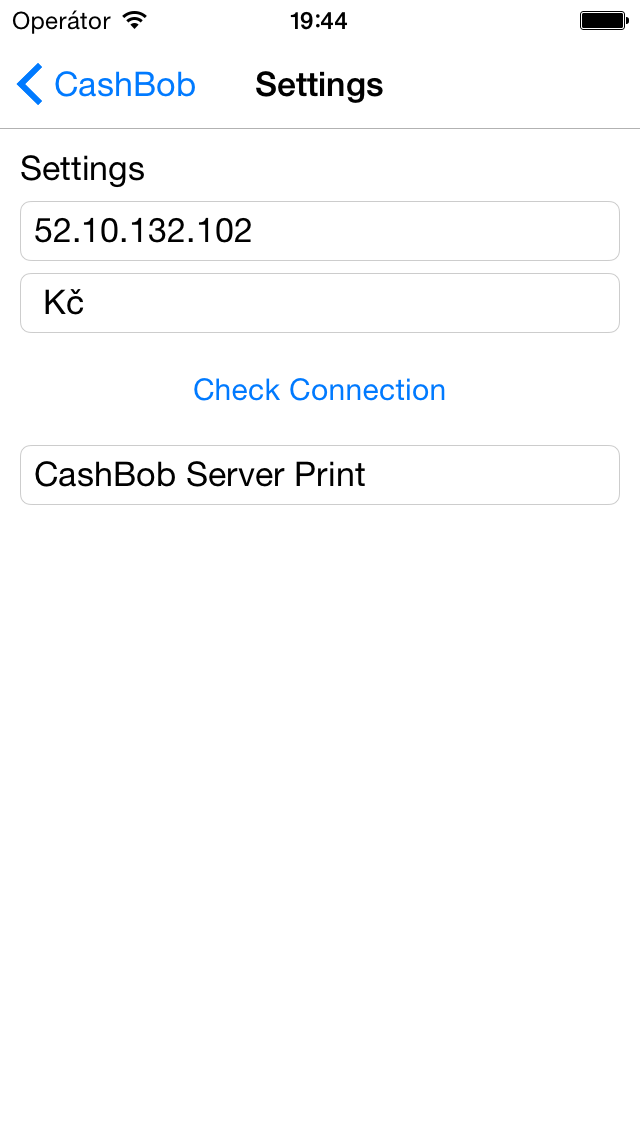
\includegraphics[width=.95\textwidth]{settings.png}
  \captionof{figure}{Nastavení}
  \label{fig:settingspage}
\end{minipage}%
\begin{minipage}{.5\textwidth}
  \centering
  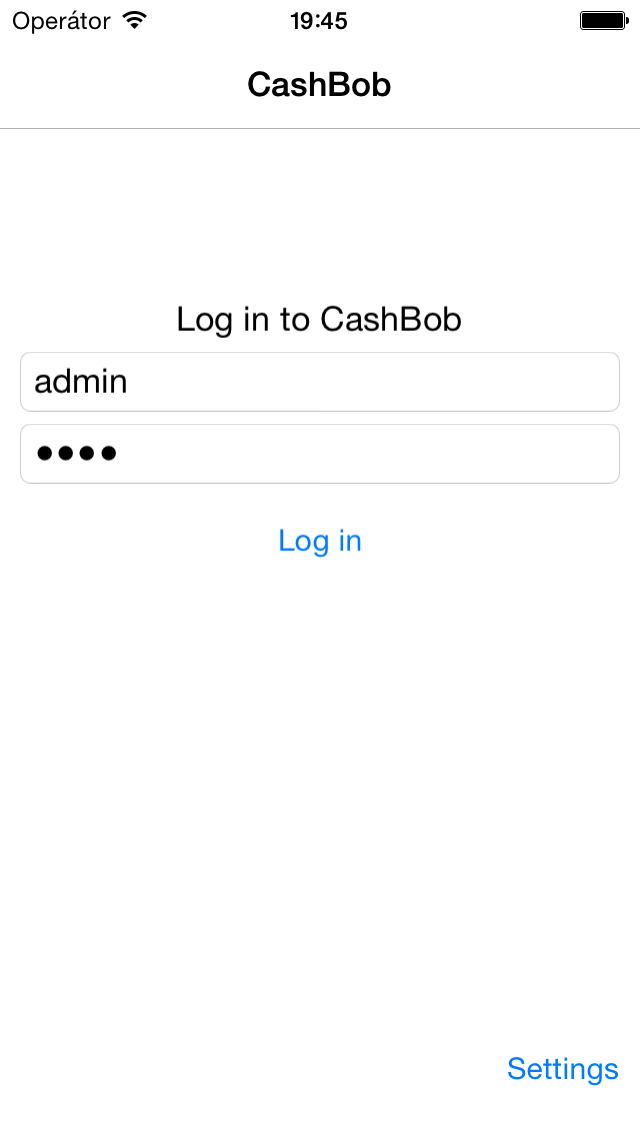
\includegraphics[width=.95\textwidth]{login.png}
  \captionof{figure}{Přihlášení}
  \label{fig:loginpage}
\end{minipage}
\end{figure}

\subsection{Připojení tiskárny Star Micronics SM-T300}
Jak zprovoznit a připojit tiskárnu k zařízení je popsáno v manuálu tiskárny, který je dostupný na \url{http://www.starmicronics.com/support/manual.aspx?printerCode=SM-T300}.
Po nabití baterie stiskněte tlačítko POWER po dobu 5 vteřin pro zapnutí tiskárny.
Potom spárujte tiskárnu se svým zařízením pomocí technologie Bluetooth.
Tiskárna se objeví pod názvem Star Micronics a PIN její 1234.
Po úspěšném spárování můžete s tiskárnou tisknout.

\subsection{Funkce aplikace}

Po přihlášení do aplikace se dostanete na stránku s existujícími účty viz obrázek \ref{fig:accountspage1}.
Jako většina stránek v aplikaci má i tato stránka vysouvací postranní panel.
Tento panel bude na telefonech schovaný a musí být vysunut tahem z levého okraje obrazovky.
Na tabletech bude vyditelný vždy pokud bude na displayi dostatek místa.
Z této stránky lze procházet účty, kterých seznam naleznete v postranním panelu viz obrázek \ref{fig:accountspage1}.
V hlavní části obrazovky je pak přehled aktivních objednávek právě zvoleného účtu jak je vidět na obrázku \ref{fig:accountspage2}.

Z této stránky jsou na horní liště nástrojů dostupné další funkce ve formě ikonek.
Ikonky nemají pod nimy popis z důvodu nedostatku místa, ale popis lze ukázat u jakékoliv ikonky v aplikaci podržením prstu na ikonce.
Jedná se o přesouvání položek mezi účty, vytvoření nového účtu, vytvoření nové objednávky na právě zvolený účet a placení položek zleva do prava. \\

\begin{figure}[h]
\centering
\begin{minipage}{.5\textwidth}
  \centering
  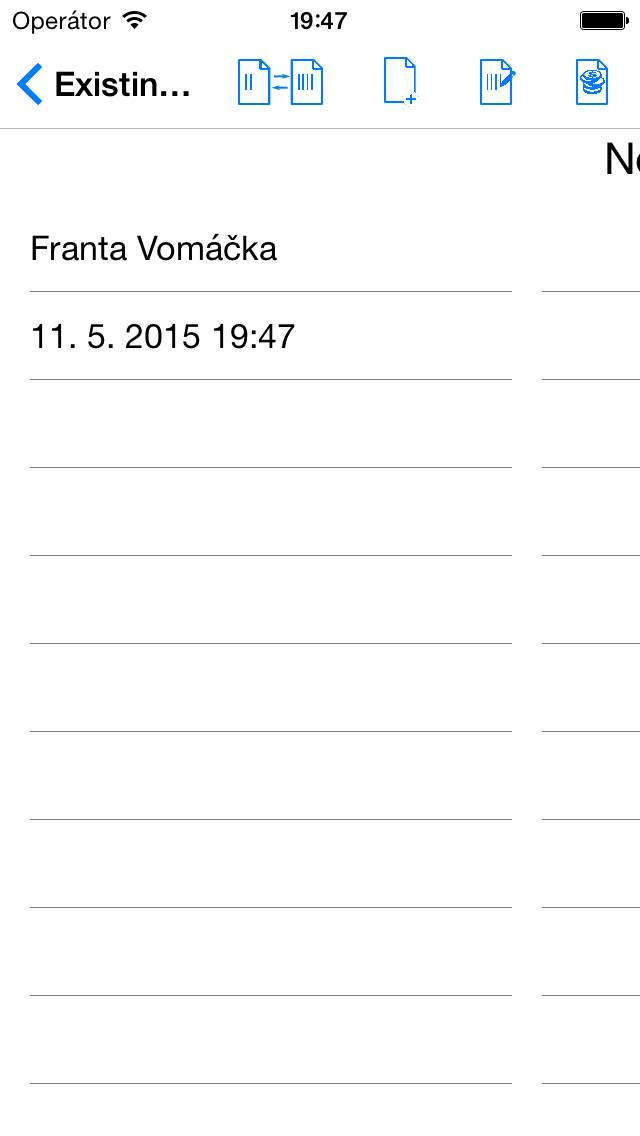
\includegraphics[width=.95\textwidth]{accounts1.png}
  \captionof{figure}{Existující účty}
  \label{fig:accountspage1}
\end{minipage}%
\begin{minipage}{.5\textwidth}
  \centering
  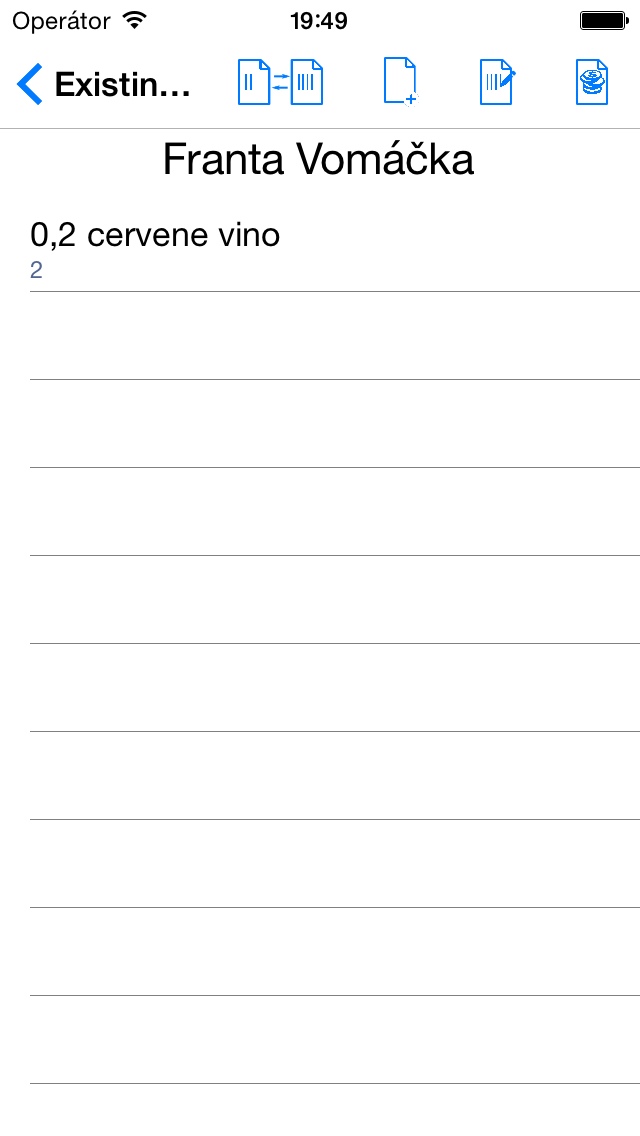
\includegraphics[width=.95\textwidth]{accounts2.png}
  \captionof{figure}{Obsah účtu}
  \label{fig:accountspage2}
\end{minipage}
\end{figure}

První z funkcí je přesun položek mezi účty.
Tato funkce se stává z dvou kroků a umožňuje přesunout aktivní objednávky z jednoho účtu na druhý.
V prvním kroku jak ukazuje obrázek \ref{fig:moveorderspage1} vybereme zdrojový a cílový účet.
Pokud cílový účet ještě neexistuje, můžeme ho vytvořit zvolením na liště nástrojů ikonky vytvořit nový účet (první ikona zleva).
Až vybereme cílový a zdrojový účet potvrdíme volbu pomocí ikonky potvrdit (druhá zleva).

V druhém kroku vybíráme které položky přesunout.
Položky volíme k přesunu pomocí tlačítka plus u dané položky.
Počet zvolených položek jednoho typu lze upravit pomocí příslušného tlačítka mínus.
V liště nástrojů jsou dostupné dvě funkce.
První z nich (zleva) potvrdí výběr, druhá automaticky přesune všechny dostupné položky.\\

\begin{figure}[h]
\centering
\begin{minipage}{.5\textwidth}
  \centering
  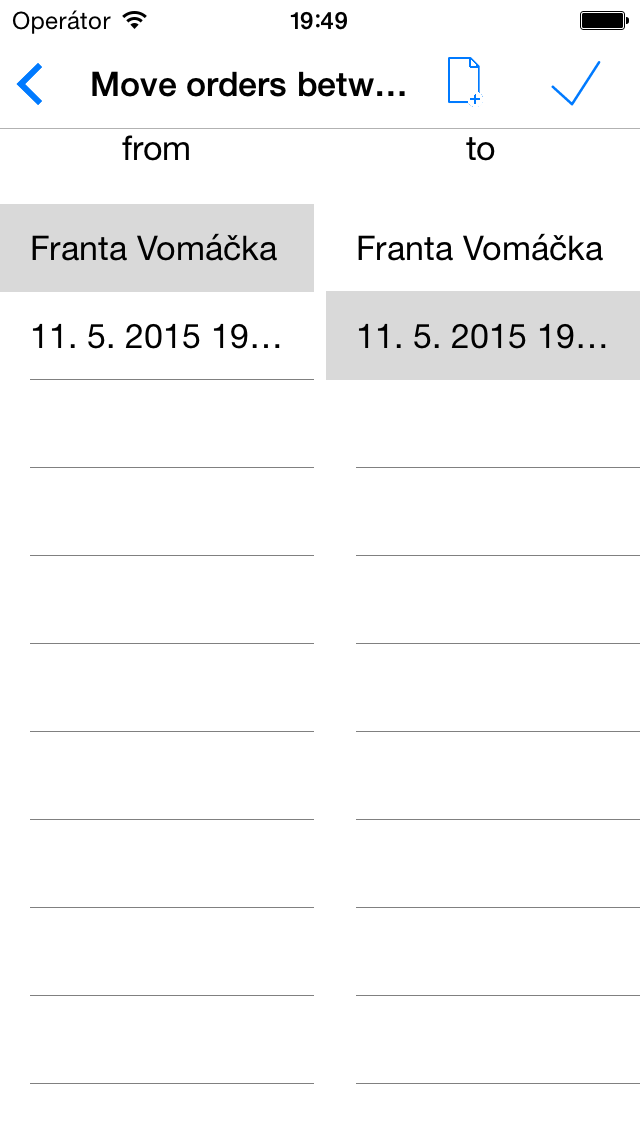
\includegraphics[width=.95\textwidth]{move1.png}
  \captionof{figure}{Přesunout položky\\ mezi účty - výběr účtů}
  \label{fig:moveorderspage1}
\end{minipage}%
\begin{minipage}{.5\textwidth}
  \centering
  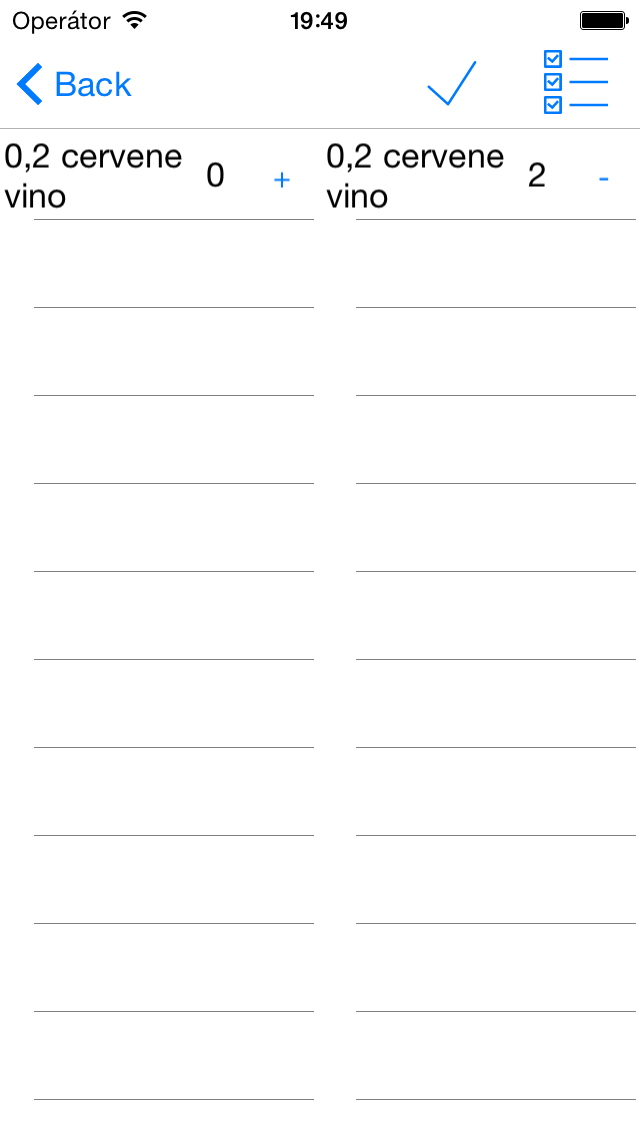
\includegraphics[width=.95\textwidth]{move2.png}
  \captionof{figure}{Přesunout položky\\ mezi účty - výběr položek}
  \label{fig:moveorderspage2}
\end{minipage}
\end{figure}

Druhou funkcí dostupnou z hlavní stránky je vytvoření nového účtu.
Tento dialog je identický pro vytváření účtu z hlavní stránky nebo ze stránky přesouvání položek.
Pokud je dialog prázdný, vypadá jako na obrázku \ref{fig:createaccountpage1}.
V tomto případě nelze vytvořit účet, protože nemá název, ale je možné vytvořit rychloobjednávku.
Tato volba vytvoří účet s časovým údajem jako názvem.
Takovýto účet je určen pro rychlé naplnění a zaplacení.

Pokud specifikujeme název, změní se tlačítko rychloobjednávka na tlačítko vytvořit.
Dále můžeme přidružit k účtu specifický stůl a napsat poznámku.\\

\begin{figure}
\centering
\begin{minipage}{.5\textwidth}
  \centering
  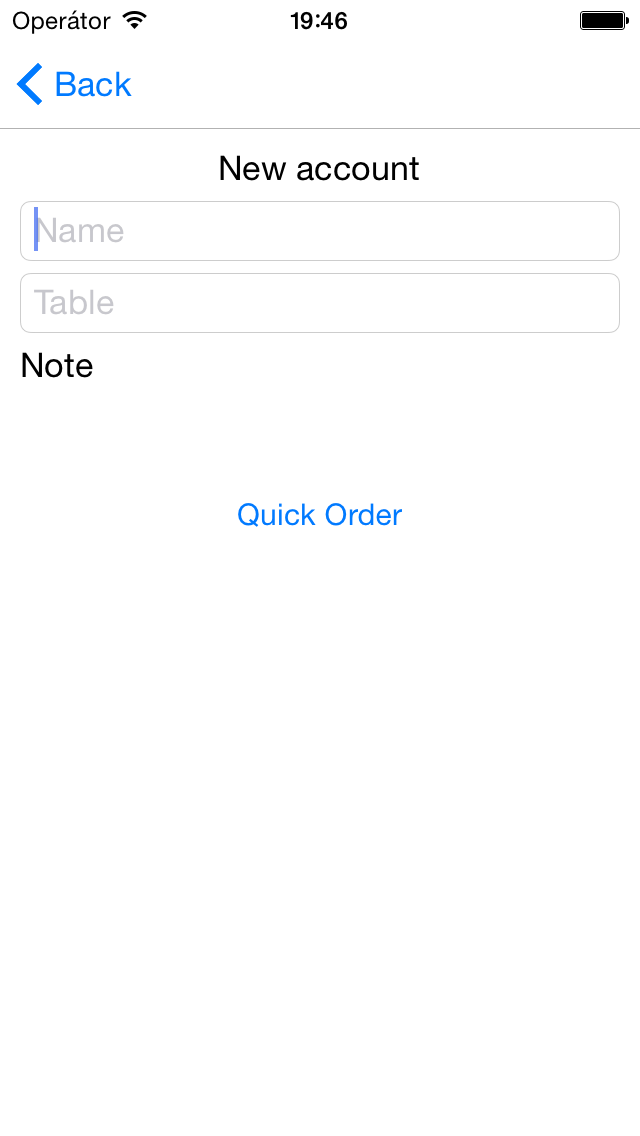
\includegraphics[width=.95\textwidth]{quickorder.png}
  \captionof{figure}{Rychloobjednávka}
  \label{fig:createaccountpage1}
\end{minipage}%
\begin{minipage}{.5\textwidth}
  \centering
  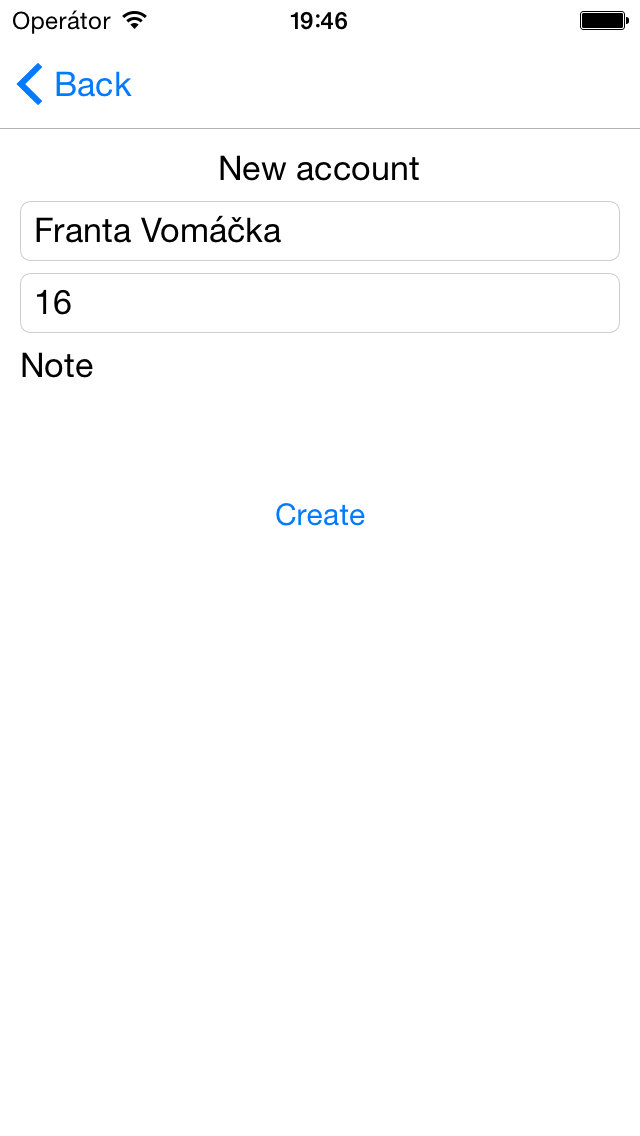
\includegraphics[width=.95\textwidth]{createaccount.png}
  \captionof{figure}{Vytvořit účet}
  \label{fig:createaccountpage2}
\end{minipage}
\end{figure}

Třetí funkcí dostupnou z hlavní stránky je vytvoření objednávky.
Jednotlivé položky dostupné k objednání jsou rozděleny do mřížkového menu (obrázek \ref{fig:createorderpage1}).
Některé položky reprezentují objednatelnou položku, jiné zas podmenu.
V tomto případě se jsou rozděleny do dvou barev: zelené a červené v tomto pořadí.
Zvolené položky se pak plní do postranního panelu viz obrázek \ref{fig:createorderpage2}.
Počet položek jednoho typu lze upravit pomocí příslušného tlačítka mínus.

V liště nástrojů jsou dostupné funkce pro navigaci stromovou strukturou menu.
Ikonky reprezentují zleva do prava přejít o úrověn nahoru, přejít do počáteční úrovně a vytvořit objednávku.\\

\begin{figure}
\centering
\begin{minipage}{.5\textwidth}
  \centering
  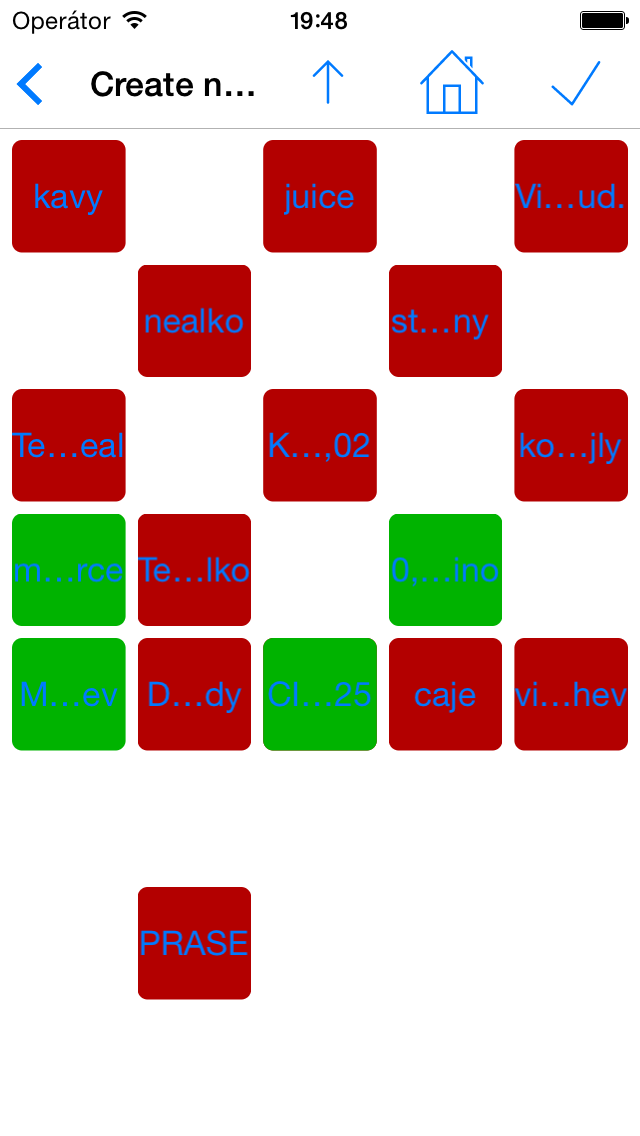
\includegraphics[width=.95\textwidth]{order1.png}
  \captionof{figure}{Vytvořit objednávku}
  \label{fig:createorderpage1}
\end{minipage}%
\begin{minipage}{.5\textwidth}
  \centering
  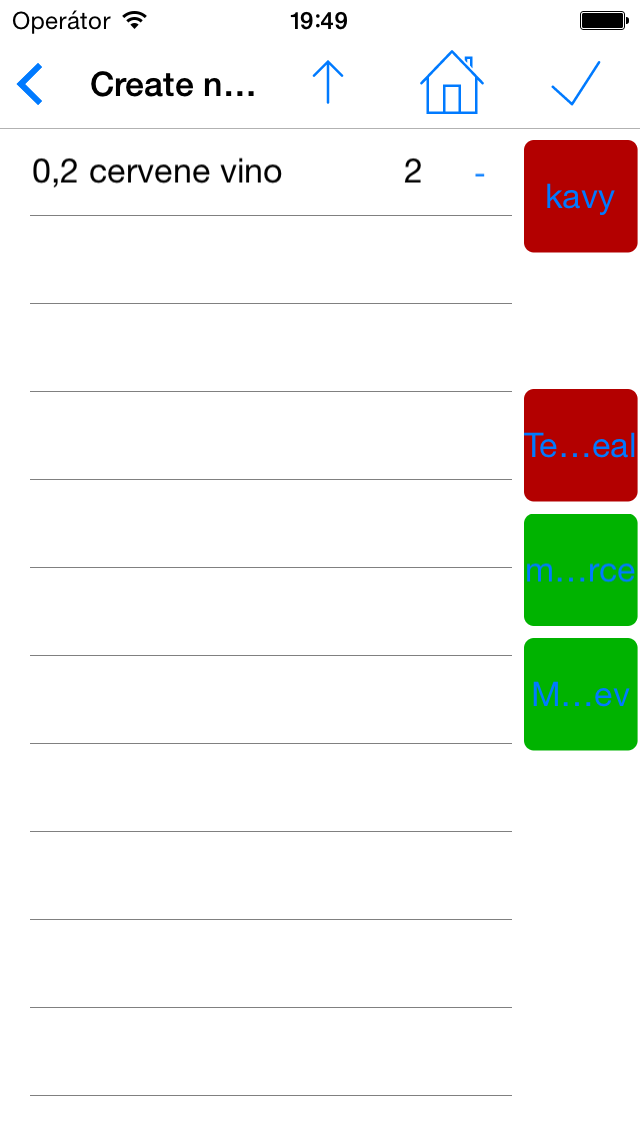
\includegraphics[width=.95\textwidth]{order2.png}
  \captionof{figure}{Vytvořit objednávku - postranní panel}
  \label{fig:createorderpage2}
\end{minipage}
\end{figure}

Poslední funkcí je platba objednávek (obrázek \ref{fig:paypage1}).
Z tohoto dialogu jsou dostupné funkce pro práci s objednávkami.
Jsou to vyčistit výběr, stornovat položky, zaplatit vybrané a zaplatit všechny.
Po vybrání položek se zobrazí druhý dialog, viz obrázek \ref{fig:paypage2}, odkud lze zkontrolovat platbu, zaplatit účet, nebo pouze vytisknout účtenku bez placení.
Poslední tlačítko placení zruší a vrátí uživatele na hlavní obrazovku.

Po zaplacení aplikace automaticky vytisk účtenku.
Pokud v nastavení není nastavena výchozí tiskárna, zobrazí se dialog s výběrem až tří možností.
Aplikace může nabídnout některé z následujících voleb, závisle na tom, které daná platforma podporuje.

\begin{itemize}

\item \textbf{Apple AirPrint}\\
    Tato volba zobrazí systémový dialog pro tisk.
    Účtenku pak lze tisknout s AirPrint kompatibilními WiFi tiskárnami.
\item \textbf{Android Print}\\
    Tato volba zobrazí systémový dialog pro tisk.
    Účtenku pak lze tisknout s podporovanými WiFi tiskárnami nebo uložit jako PDF.
\item \textbf{CashBob Server Print}\\
    Tato volba pošle žádost aplikaci CashBob Server na počítač, která vytiskne účtenku na výchozí tiskárnu počítače.
    Tuto funkci nelze využít s cloudovým serverem, protože k němu není připojená žádná tiskárna.
\item \textbf{Star Portable Printer}\\
    Tato volba umožňuje tisk s mobilní tiskárnou Star Micronics SM-T300.
    Tiskárna musí být připojena k zařízení přes Bluetooth, aby mohla být účtenka vytisknuta.
\end{itemize}

\begin{figure}
\centering
\begin{minipage}{.5\textwidth}
  \centering
  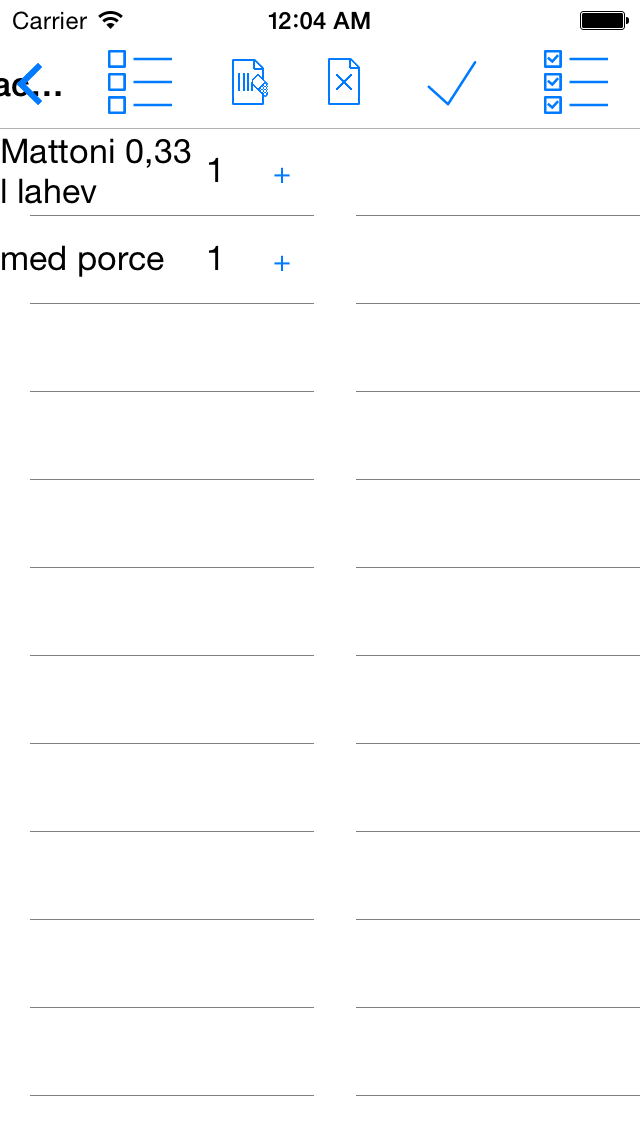
\includegraphics[width=.95\textwidth]{pay1.png}
  \captionof{figure}{Zaplatit - výběr položek}
  \label{fig:paypage1}
\end{minipage}%
\begin{minipage}{.5\textwidth}
  \centering
  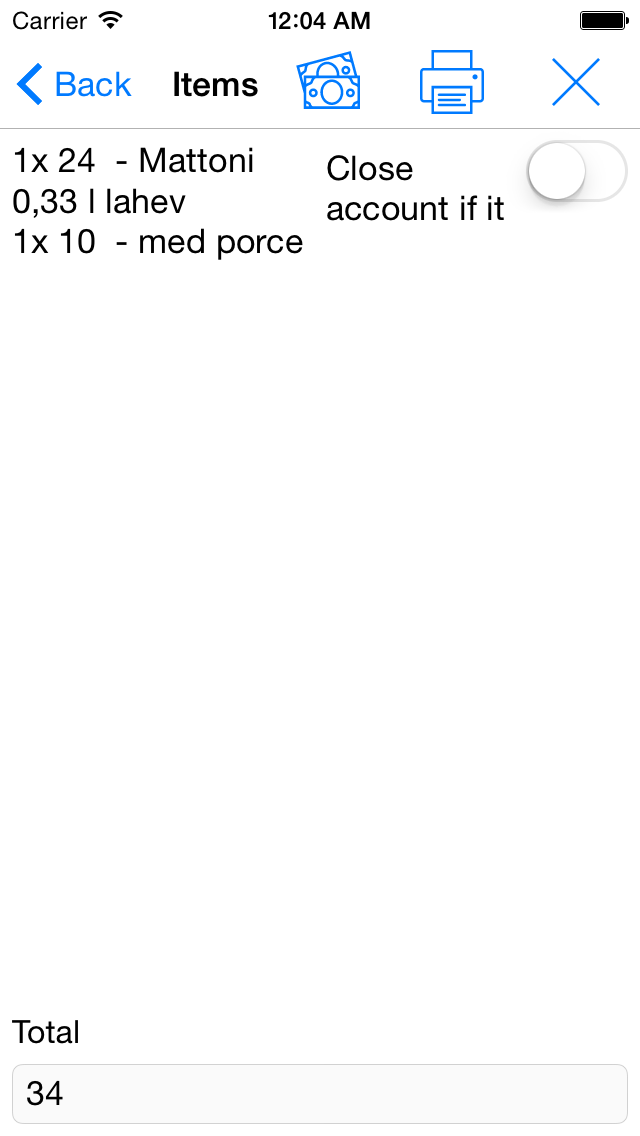
\includegraphics[width=.95\textwidth]{pay2.png}
  \captionof{figure}{Zaplatit - potvrzení}
  \label{fig:paypage2}
\end{minipage}
\end{figure}
\chapter{CD Contents}
\label{ch:cdcontents}

\begin{itemize}
\item \textbf{/Bin}
    \begin{itemize}
    \item \textbf{CashBob.Mobile.apk} - instalační balíček mobilní aplikace CashBob pro operační systém Android
    \item \textbf{CashBobServer.zip} - archiv s aplikací CashBob Server
    \item \textbf{CashBobClient.zip} - archiv s aplikací CashBob Client
    \end{itemize}
    
\item \textbf{/Source}
    \begin{itemize}
    \item \textbf{/CashBob.Mobile} - zdrojové kódy mobilních aplikací
    \item \textbf{/CashBob} - zdrojové kódy systému CashBob
    \end{itemize}
\item \textbf{/Doc}
    \begin{itemize}
    \item \textbf{/Design} - grafické produkty této práce
    \item \textbf{/Thesis} - zdrojové soubory textové části práce (\LaTeX)
    \item \textbf{/Documentation} - vygenerovaná HTML dokumentace k mobilní aplikaci
    \item \textbf{manual.pdf} - samostatná instalační a uživatelská příručka
    \item \textbf{drykjan\_2015bach.pdf} - text bakalářské práce ve formátu PDF
    \item \textbf{vykaz.xlsx} - Výkaz práce ve formátu aplikace  Microsoft Excel
    \end{itemize}

\item \textbf{/Video}
    \begin{itemize}
    \item \textbf{uitest.mp4} - Video-ukázka probíhajícího UI testu
    \end{itemize}
\item \textbf{readme.txt} - textový soubor s popisem obsahu CD
\end{itemize}

\end{document}
